\documentclass[a4paper]{article}
\usepackage{cmap}					% поиск в PDF
\usepackage[T2A]{fontenc}			% кодировка
\usepackage[utf8]{inputenc}			% кодировка исходного текста
\usepackage[english,russian]{babel}	% локализация и переносы

\usepackage{tikz}

\usepackage{bm}
\usepackage{amsmath,amsfonts,amssymb,amsthm,mathtools} % AMS
\usepackage{icomma}

\usepackage{xcolor}
\usepackage{array}
\usepackage{svg}

\usepackage[colorlinks=true]{hyperref}

\usepackage[left=3cm,right=1cm,top=2cm,bottom=2cm,bindingoffset=0cm]{geometry}
\linespread{1.3}

\newcolumntype{C}[1]{>{\centering\arraybackslash}p{#1}}


\begin{document}
	
\section{Формулировка задания}
Целью данной работы является проектирование базы данных для индексирования геоданных: оптических и радарных космических снимков, а так же соответствующих им векторных масок; с целью дальнейшего их использования в создании алгоритмов машинного обучения и новых масок.
При создании базы данных необходимо учитывать типовые операции, проводящиеся со снимками в рамках процесса разработки алгоритмов, а так же обеспечить расширяемость на новые типы снимков.

\section{Описание предметной области}
Многие практические задачи обработки ДЗЗ, такие как сегментация подстилающей поверхности, устранение дефектов снимков, улучшение разрешения и т.д., не могут быть решены классическими алгоритмами обработки. Поэтому, всё чаще используются алгоритмы на основе машинного обучения, причём, как правило, типа ``supervised learning''.
Данные алгоритмы требуют больших объёмов тренировочных (размеченных) данных, например для сегментации поверхности --- это созданные вручную маски поверхности.
Для того, чтобы оптимизировать время разработки новых моделей, требуется наладить конвейер обработки данных и моделей.
В рамках этой работы рассмотрено проектирование базы данных для такого конвейера.

\subsection{Некоторые определения}
\begin{itemize}
	\item Продукт --- совокупность одного или нескольких снимков, обладающих некоторыми общими свойствами.
		Например: стереопары --- это пары снимков одной территории, снятые примерно в одно время с разных ракурсов (углов).
		Позволяют строить стереомодели объектов.
	\item Выборка --- совокупность продуктов, и, иногда, векторных масок к ним, отобранная для обучения или тестирования алгоритма.
	\item Сенсор --- в узком смысле --- спутник, производящий съемку.
		В широком смысле --- система спутников одного вида, обладающих одинаковыми свойствами (например --- пространственным разрешением).
	\item Векторная маска / разметка / вектор --- полигон или множество полигонов, имеющих географическую привязку, и описывающих какие-то объекты / типы территории на снимках.
\end{itemize}

\subsection{Типовые операции с данными}
\subsubsection{Тематический отдел}
Тематический отдел занимается созданием разметки.
Типовые операции тематического отдела:
\begin{itemize}
	\item Получение продукта по географическим координатам от определённого сенсора за определённый временной промежуток.
	\item Получение продукта по исходному идентификатору.
	\item Добавление новой векторной маски.
	\item Получение стабильной версии модели машинного обучения для произведения полуавтоматической разметки.
	\item Добавление свойств продукта.
	\item Формирование выборки.
\end{itemize}

\subsubsection{Алгоритмический отдел}
Алгоритмический отдел занимается созданием алгоритмов для обработки.
Типовые операции алгоритмического отдела:
\begin{itemize}
	\item Формирование выборки (иногда).
	\item Получение, первичная обработка выборки.
	\item Добавление новых моделей машинного обучения.
	\item Добавление новых версий моделей машинного обучения.
	\item Отслеживание версий экспериментов (интеграция с VCS, например с GIT).
\end{itemize}

\section{Модели базы данных}
\subsection{Концептуальная модель БД}
На основе приведённых выше типовых операций, а так же общей структуры предметной области, была составлена концептуальная модель БД.
Для того, чтобы не засорять схему, атрибуты не были указаны на ней, а вместо этого представлены в разделе \nameref{attributes_definitions}

\begin{figure}[h]
	\centering
	\includesvg[width=\columnwidth]{./images/ER.svg}
	\caption{Концептуальная модель БД}
\end{figure}

\subsection{Список сущностей}
В ходе моделирования, были выделены следующие сущности:
\begin{itemize}
	\item Продукт
	\item Снимок
	\item Источник
	\item Снимок НЦОМЗ
	\item Снимок ``Planet''
	\item Снимок ``DG''
	\item Вектор
	\item Автор
	\item Обработчик
	\item Выборка
	\item Модель
	\item Эксперимент
	\item Класс вектора
\end{itemize}

\subsection{Описание атрибутов}
\label{attributes_definitions}
В следующих таблицах приводится более подробное описание атрибутов каждой сущности.

\begin{table}[h]
	\begin{tabular}{|C{0.20\textwidth}|p{0.75\textwidth}|}
		\hline
		Атрибут & \centering\arraybackslash Описание \\
		\hline
		type & Тип продукта. На данный момент всего два типа: стерео и обычный, но может значительно пополняться в будущем \\
		\hline
		images & Множество снимков, входящих в данный продукт \\
		\hline
		delivery\_id & Номер поставки, нужен для отслеживания в случае обнаружения некорректных поставок \\
		\hline
		indexed\_datetime & Время добавления в БД \\
		\hline
	\end{tabular}
	\caption{Описание атрибутов продукта}
\end{table}

\begin{table}[h]
	\begin{tabular}{|C{0.20\textwidth}|p{0.75\textwidth}|}
		\hline
		Атрибут & \centering\arraybackslash Описание \\
		\hline
		name & Название данного источника \\
		\hline
		additional\_fields & Список полей (атрибутов), не входящих в сущность ``Снимок'', но присутствующих в отдельной таблице снимков для этого источника. Например, cloud\_map для ``Planet'' \\
		\hline
	\end{tabular}
	\caption{Описание атрибутов источника снимка}
\end{table}

\begin{table}[h]
	\begin{tabular}{|C{0.20\textwidth}|p{0.75\textwidth}|}
		\hline
		Атрибут & \centering\arraybackslash Описание \\
		\hline
		id & Внутренний идентификатор снимка (так же первичный ключ) \\
		\hline
		external\_id &  Внешний идентификатор снимка (используется для индексации снимков в системе, откуда он был получен) \\
		\hline
		source & Источник, из которого был получен снимок \\
		\hline
		sat & Спутника с которого был получен снимок \\
		\hline
		capture\_conditions & Дополнительные параметры съёмки: угол наклонения орбиты, солнца и т.д. \\
		\hline
		captured\_datetime & Дата и время, в которое был сделан снимок (усреднённое значение) \\
		\hline
		processed\_datetime & Дата и время, когда снимок был обработан во внешней системе обработки \\
		\hline
		type & Тип снимка: мультиспектральный, панхроматический, или результат паншарпенинга \\
		\hline
		geometry & Геометрия снимка на поверхности земли (геопривязка) \\
		\hline
		path & Путь к самому снимку \\
		\hline
		ql\_path & Путь к снимку сжатому в несколько раз, для быстрого ``поверхностного'' просмотра \\
		\hline
		other\_paths & Пути к другим файлам, которые шли в поставке вместо со снимком \\
		\hline
	\end{tabular}
	\caption{Описание атрибутов снимка}
\end{table}

\begin{table}[h]
	\begin{tabular}{|C{0.20\textwidth}|p{0.75\textwidth}|}
		\hline
		Атрибут & \centering\arraybackslash Описание \\
		\hline
		cloud\_map & Полигон, описывающий облака и тени от облаков, присутствующие на снимке \\
		\hline
	\end{tabular}
	\caption{Описание атрибутов снимка ``Planet''}
\end{table}

\begin{table}[h]
	\begin{tabular}{|C{0.20\textwidth}|p{0.75\textwidth}|}
		\hline
		Атрибут & \centering\arraybackslash Описание \\
		\hline
		cloud\_map & Полигон, описывающий облака и тени от облаков, присутствующие на снимке \\
		\hline
		stereo\_number & Номер стереоснимка (если тип продукта стерео), иначе -1 \\
		\hline
	\end{tabular}
	\caption{Описание атрибутов снимка ``DG''}
\end{table}

\begin{table}[h]
	\begin{tabular}{|C{0.20\textwidth}|p{0.75\textwidth}|}
		\hline
		Атрибут & \centering\arraybackslash Описание \\
		\hline
		hash & Уникальный хэш первичной обработки снимка \\
		\hline
		scene & Номер сцены в пролёте \\
		\hline
		selected & Является ли данный снимок ``отобранным'' --- т.е. приемлемым для работы \\
		\hline
		defects & Список дефектов данного снимка \\
		\hline
	\end{tabular}
	\caption{Описание атрибутов снимка НЦОМЗ}
\end{table}


\begin{table}[h]
	\begin{tabular}{|C{0.20\textwidth}|p{0.75\textwidth}|}
		\hline
		Атрибут & \centering\arraybackslash Описание \\
		\hline
		datetime & Дата и время создания данного вектора \\
		\hline
		authors & Множество сущностей (людей и других алгоритмов), принимавших участие в создании вектора \\
		\hline
		class & Класс, который выделен данным вектором \\
		\hline
		image & Изображение, на которое был создан данный вектор \\
		\hline
		other & Дополнительные поля \\
		\hline
		geometry & Непосредственно полигоны, задающие данный вектор \\
		\hline
	\end{tabular}
	\caption{Описание атрибутов вектора}
\end{table}

\begin{table}[h]
	\begin{tabular}{|C{0.20\textwidth}|p{0.75\textwidth}|}
		\hline
		Атрибут & \centering\arraybackslash Описание \\
		\hline
		short\_description & Краткое описание данного класса вектора. Например: лес, озеро, дефект матрицы и т.д. \\
		\hline
		description & Полное описание данного класса. Например: ``Дефект матрицы 2-го типа, обычно вызванный внутренними перебоями питания КА'' \\
		\hline
		color & Цвет, которым нужно выделять данный класс на ситуационной карте \\
		\hline
	\end{tabular}
	\caption{Описание атрибутов класса вектора}
\end{table}


\begin{table}[h]
	\begin{tabular}{|C{0.20\textwidth}|p{0.75\textwidth}|}
		\hline
		Атрибут & \centering\arraybackslash Описание \\
		\hline
		name & ФИО автора \\
		\hline
		contacts & Каналы для связи \\
		\hline
	\end{tabular}
	\caption{Описание атрибутов автора}
\end{table}


\begin{table}[h]
	\begin{tabular}{|C{0.20\textwidth}|p{0.75\textwidth}|}
		\hline
		Атрибут & \centering\arraybackslash Описание \\
		\hline
		images & Список снимков в данной выборке \\
		\hline
		masks & Список векторных масок в данной выборке \\
		\hline
		parent & Родительская выборка. Выборки образуют структуру похожую на лес, т.е. множество деревьев \\
		\hline
	\end{tabular}
	\caption{Описание атрибутов выборки}
\end{table}


\begin{table}[h]
	\begin{tabular}{|C{0.20\textwidth}|p{0.75\textwidth}|}
		\hline
		Атрибут & \centering\arraybackslash Описание \\
		\hline
		author & Автора эксперимента \\
		\hline
		datetime & Время начала эксперимента \\
		\hline
		git\_commit & Хэш коммита в VCS, отвечающий данному эксперименту \\
		\hline
		dataset & Выборка, использовавшаяся в данном эксперименте \\
		\hline
		parent & Родительский эксперимент (эксперименты образуют структуру типа леса, т.е. множества деревьев) \\
		\hline
		models & Список моделей, порождённых данным экспериментом \\
		\hline
	\end{tabular}
	\caption{Описание атрибутов эксперимента}
\end{table}


\begin{table}[h]
	\begin{tabular}{|C{0.20\textwidth}|p{0.75\textwidth}|}
		\hline
		Атрибут & \centering\arraybackslash Описание \\
		\hline
		type & Тип модели: сегментация, детекция, регрессия и т.д. \\
		\hline
		paths & Список путей к файлам модели (обученная модель представляет из себя бинарный файл, но может быть сохранена в разных форматах, иногда без возможности конвертации между ними) \\
		\hline
		other & Дополнительные атрибуты \\
		\hline
	\end{tabular}
	\caption{Описание атрибутов модели}
\end{table}

\subsection{Логическая модель БД}
Следующим шагом было построение логической модели БД, подробнее отражающей реализацию концепции в рамках реляционной модели.
Связи типа ``многие-ко-многим'' реализованы с помощью отдельных связующих таблиц.
Связи типа ``один-к-одному'' реализованы с помощью техники выносного первичного ключа.
Древовидные структуры (эксперименты и выборки) реализованы с помощью хранения ссылки на родительский элемент.

\begin{figure}[h]
	\centering
	\includesvg[width=\columnwidth]{./images/Logic.svg}
	\caption{Логическая модель БД}
\end{figure}


\subsection{Физическая модель БД}
В качестве СУБД для реализации была выбрана PostgreSQL.
Основным фактором при выборе СУБД было наличие средств / библиотек для работы с геометрическими типами данных.
В PostgreSQL такой инструмент есть и является очень хорошо развитым.
PostGIS позволяет эффективно осуществлять геометрические запросы, например по пересечению, объединению, вхождению и т.д.
Кроме того, в PostGIS в виде хранимых процедур реализованы и другие функции для работы с геометрией: перепроецирование, нахождение площади произвольных полигонов и т.д.

\begin{figure}[h]
	\centering
	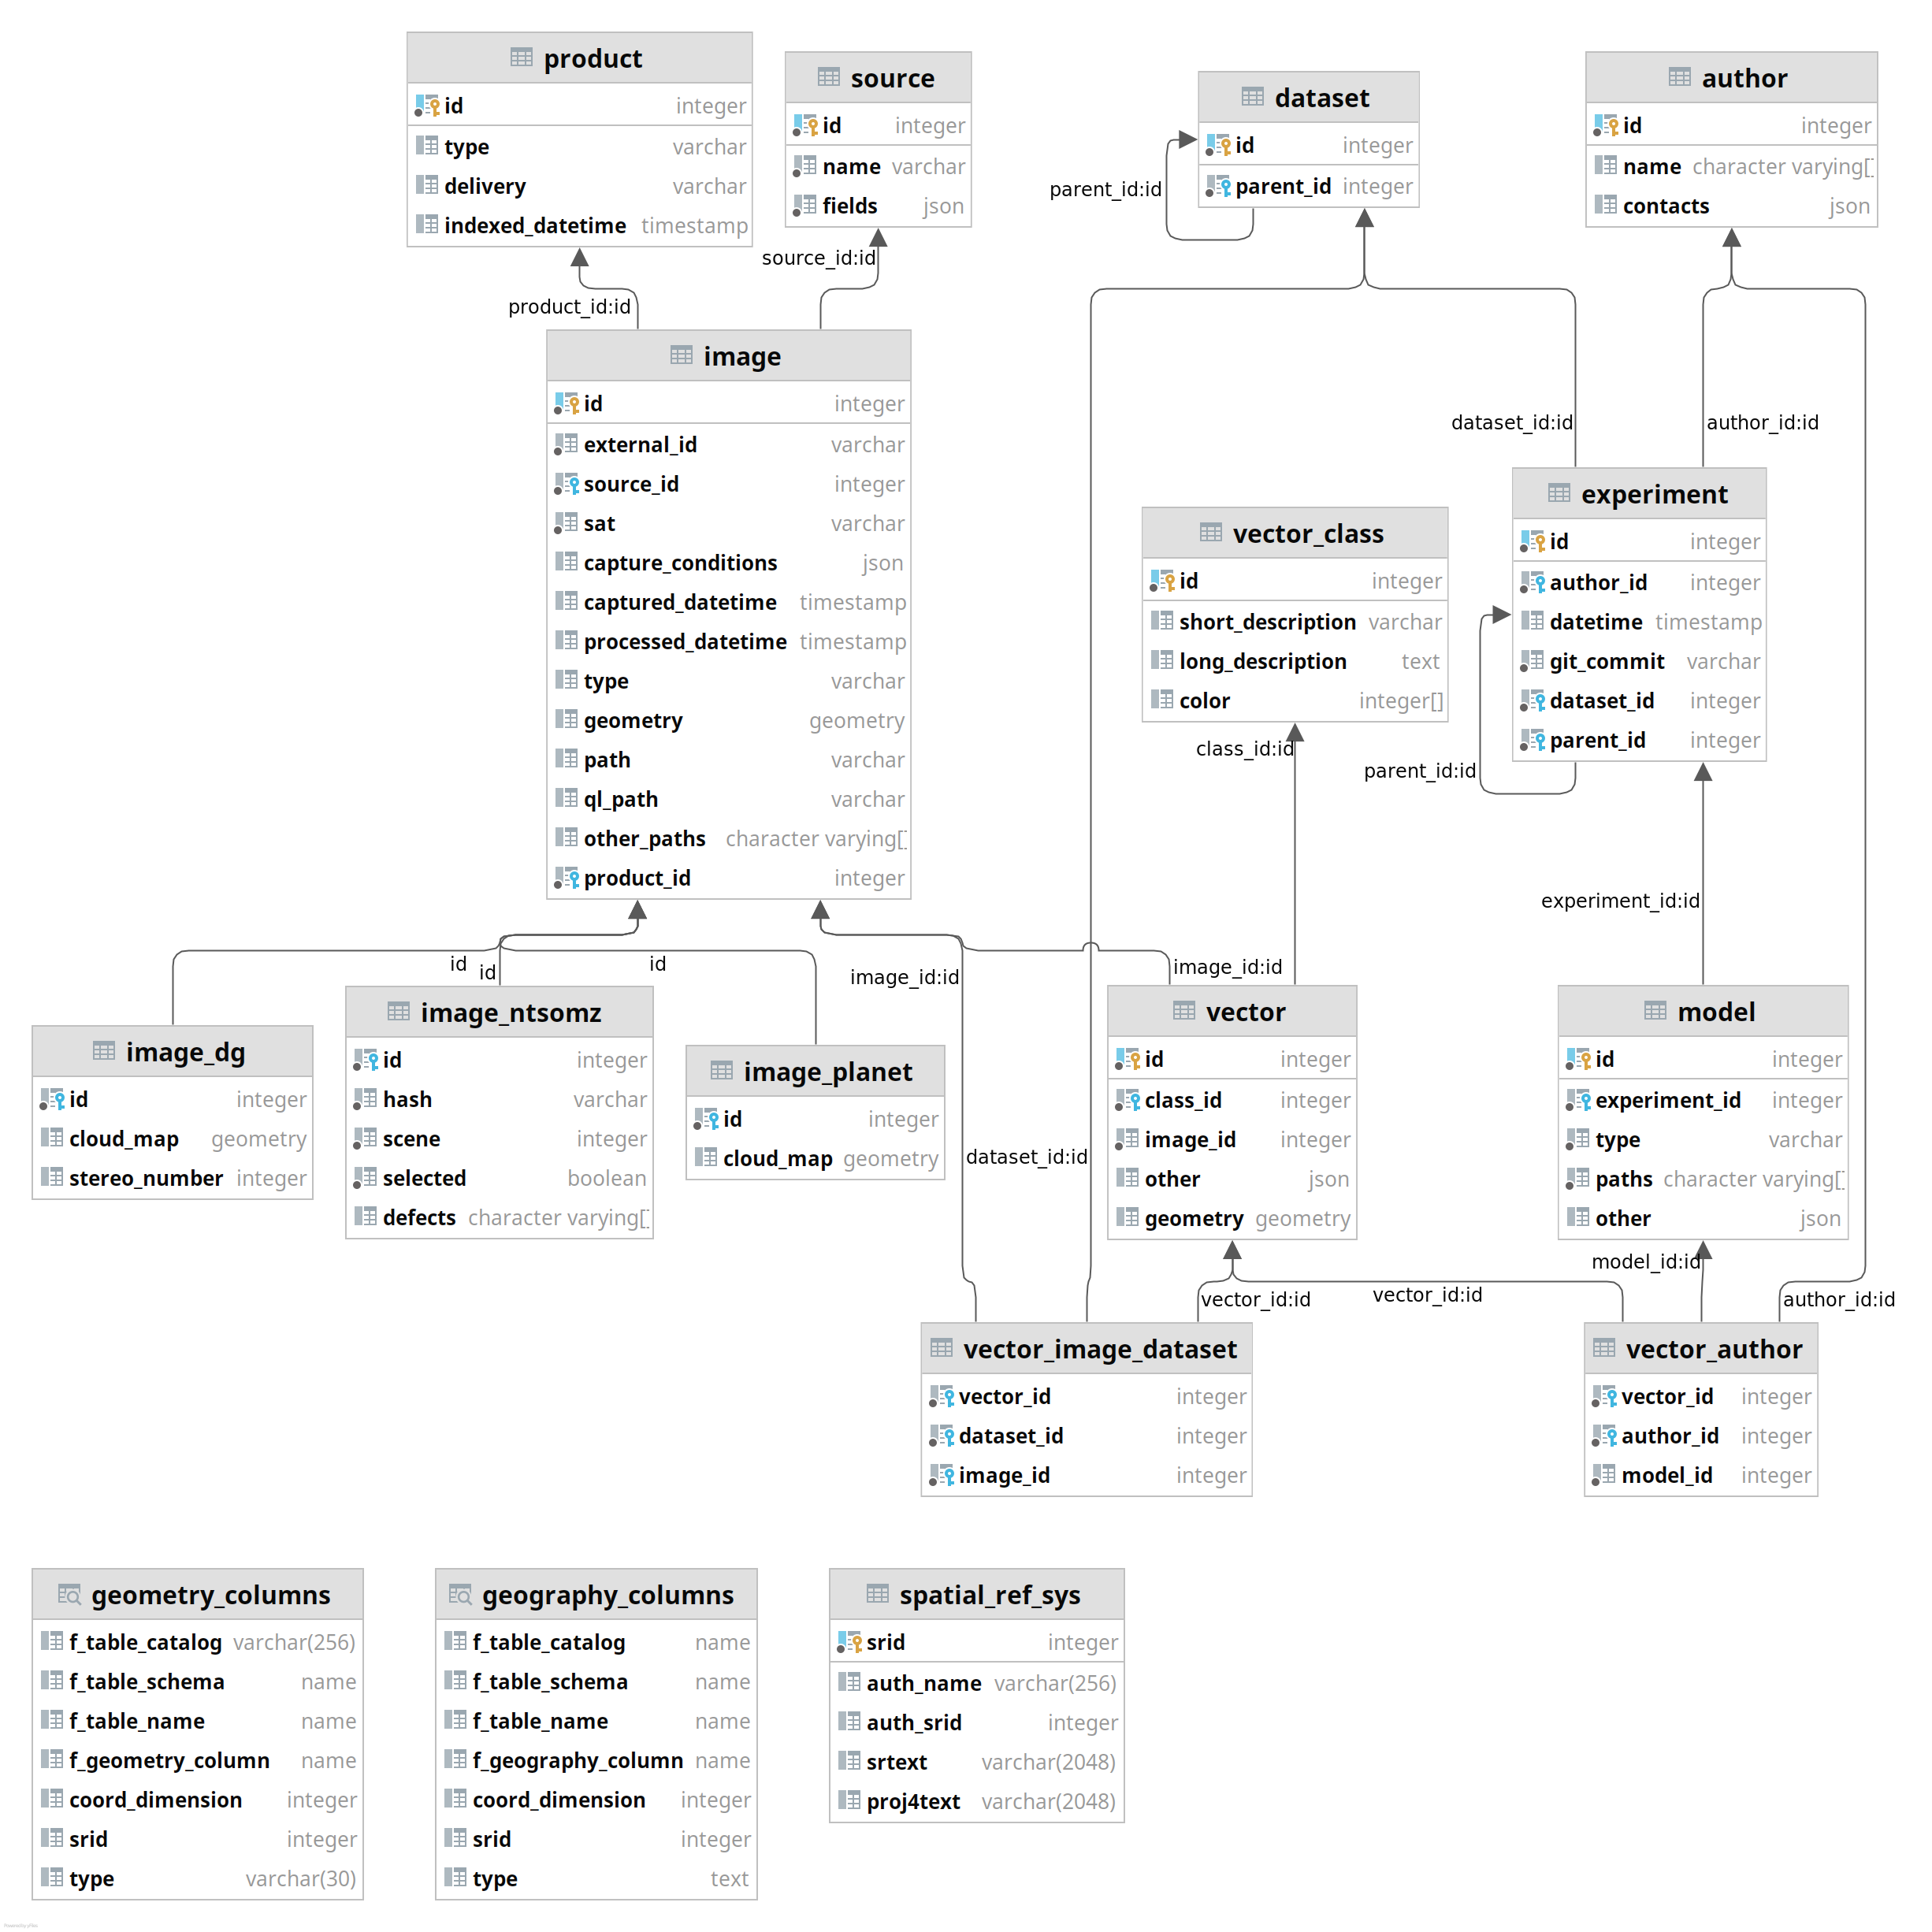
\includegraphics[width=\columnwidth]{./images/Physics.png}
	\caption{Физическая модель БД в СУБД PostgreSQL}
\end{figure}


	
\end{document}